\chapter{How some stuff works}%
\label{cha:how_stuff_works}

This section describes in detail some areas of \CGG{} to help explain how things work.

\section{Copy/Paste and Highlight Usage}%
\label{sec:copy_paste_highlight_usage}

There are 3 types of copy/cut and paste methods which exist in X windows, and most modern programs use 2 of them.  The 3 cases are:

\begin{description}
    \item[cut\_buffers 0-7] these are obsolete but they still work and are the simplest to use.
    \item[highlighting] called primary selection; almost all clipboard programs only use this.
    \item[copy and paste] called secondary (or clipboard) selection. Some more modern programs use Ctrl-C/Ctrl-X and Ctrl-V for this (some use other keys or qualifiers, like Shift).
\end{description}

\subsection*{How it works:}%
\label{sub:how_it_works}

All of the methods use window \textit{properties} to attach data, called a selection, to a source window.  The program advertises the selection by using the X server.  The window property used determines which selection type is set/advertised by the new selection.

When a paste is used in a target window, the target program requests the advertised selection data.  This may access one of two buffers depending on which type of load/paste action is used.  The user loads a \textit{cut buffer} via Drag select or Ctrl-C/Ctrl-X, and pastes a \textit{cut buffer} via middle mouse press or Ctrl-V.

\subsection*{\CGG{} cut and paste:}%
\label{sub:cinelerra_cut_paste}

\subsubsection*{1. Text cut and paste operations}%
\label{ssub:text_cut_paste_operations}

To use a text selection, create a drag selection in textboxes by pressing and holding left mouse button with the pointer over the beginning of the text selection, then move the pointer over the desired selection to the selection end, then release the mouse button.  This continuously reloads the \textit{primary} clipboard buffer and highlights the text selection.  It can then be pasted to most programs by pressing the middle mouse button with the pointer over the text insertion point.  Some examples of these programs are \textit{xterm}, \textit{gnome-terminal}, \textit{cinelerra}, and \textit{browser} input text boxes.  After you create a text selection, if you then press Ctrl-C the selection will also be copied to the \textit{secondary} (or \textit{clipboard}) selection buffer.  This second paste buffer can be used for a more lasting save effect, since it will not be lost until you again press Ctrl-C (copy).  Using Ctrl-V (cut) will also copy the selection to the secondary clipboard buffer, and then delete the selection from the textbox.  If you press Ctrl-V (or paste) in a target window, the secondary selection will be inserted at the target window cursor.  If a text selection exists in the target window, it is replaced by the pasted text.

\subsubsection*{2. Media cut and paste operations}%
\label{ssub:media_cut_paste_operations}

To create a media selection, highlight a region on the \CGG{} media timeline, then use the main menubar or compositor/viewer edit panel to operate the clip cut, copy, or copy-keyframe menu buttons.  This selection can then be pasted to a target selection on the timeline using the main menubar or compositor/viewer edit panel to operate the clip paste or paste-keyframe operation.  Also, by using the resource window you can select the \textit{Clips} folder and right mouse the resources list box, then use the \textit{Paste Clip} menu item to paste the selection to a named clip.  Additionally, these methods work between running instances of \CGG{}, which means you can move media clips between the \CGG{} program instances.  The clip data is also copied to the secondary clipboard buffer.  This makes it possible to examine the clip content directly if so desired.

\subsubsection*{3. The older cut\_buffer method}%
\label{ssub:older_cut_buffer_method}

\begin{itemize}
    \item For text, if there is an active selection when a window closes, it uses \texttt{cut\_buffer0}.  Normally when a paste is performed, the target window \textit{notifies} the selection owner to \textit{send it now} when you do a paste, but if the window has closed there is no source window, so no pasting.  Some programs, like \CGG{}, use \texttt{cut\_buffer0} as a fallback.  This makes it possible to paste data from a closed window.
    \item To move media clip, data \texttt{cut\_buffer2} is used because it does not require the selection owner interface, and works simply and reliably.  This buffer is not normally in use by other programs.
\end{itemize}

\subsection*{Final note}%
\label{sub:final_note}

When a text selection is set, the selected text is redrawn using selected-highlight color when the textbox loses focus.  This convenience feature shows the active text selection as you move the pointer to the new target window.  When a new selection is set anywhere else on your screen, the current text selection will be redrawn using the inactive-highlight color as the textbox loses selection ownership.  In most \CGG{} themes, the drag selection text-highlight color is BLUE ($\#0000FF$), the selected-highlight color is SLBLUE ($\#6040C0$) -- really sort of purple, and the inactive-highlight color is MEGREY ($\#AFAFAF$).

\section{Playing is Different than Seeking/Positioning!}%
\label{sec:playing_seeking_positioning}

\subsection{Playing/Seeking}%
\label{sub:playing_seeking}

\textit{Seeking} targets and displays the next frame.  The next frame is targeted because frame zero has no previous.  When you seek, you reposition to just before the target frame, and since the play direction has not been established (there is no direction when seeking) it shows you the next frame.  This produces the expected behavior when you seek to frame zero; you see the first frame.  Seeking displays in the compositor what you are getting ready to work with/edit/etc; always showing the next frame in relation to the cursor. Technically, since seeking just resets the position, it would be correct not to update the compositor, but it is best to seek and show the next frame to confirm that it is the frame you expected to see.

\textit{Playing} shows you what has just been played in the compositor window.  It is not the same as seeking. When you use Keypad 1 to play frame forward, then the 1st frame that is played and shown in the compositor window is frame zero (which was already displayed).  The position is incremented to 1.  Press Keypad 1 yet again, and the next frame displayed is 1, and the new position is 2, and so on.  According to the implemented strategy, the insertion point moves to track playback.  When playback stops, the insertion point stays where playback stopped.  Thus, with playback you change the position of the insertion point.

Simple explanation of what you will be seeing in the compositor when playing:

\begin{description}
    \item[Play forward] the frame to the right of the cursor in the timeline gets displayed.
    \item[Play backward] the frame to the left of the cursor in the timeline gets displayed.
\end{description}

The reason behind this \textit{play} methodology is that you want to know what you just played so that you know what matches what you just saw/heard in case that is the desired stuff.   You don't want the compositor to show you what you have not yet played -- you need to see this frame to analyze/check to see if it is what you want.  This behavior applies to any playing operation, such as the \textit{keypad} or \textit{Frame forward / Frame reverse} buttons.  You can still easily see the actual insertion point in the zoombar at the bottom of the timeline -- sixth button over or 3rd button from the right side.   Also note the following:

\begin{description}
    \item[Blinking insertion point on the timeline] seeking/positioning was the last operation.
    \item[Solid non-blinking insertion point on timeline] playing was the last operation.
\end{description}

\subsubsection*{Example and explanation}%
\label{ssub:example_explanation}

\begin{enumerate}
    \item open a small example of 10 numbered frames (or use the \texttt{Title} plugin to add a timestamp)
    \item press "f" to \textit{fit} the timeline
    \item make sure \texttt{settings $\rightarrow$ align\_cursor\_on\_frames} is set
    \item seek to frame 4 by clicking on the timeline at position 4, compositor shows the 5th frame, since the
    media counts from 1 and the timeline counts from 0.  This is correct behavior.
    \item press KP1 to play next frame.  According to playback strategy: \textit{When play is forwards, the next unit is displayed, and the position is advanced one unit}. So the next frame is 4, (shows the $5^{th}$ frame) it is displayed. The position is advanced from 4 to 5.  This is correct behavior.
    \item press KP4 to play the previous frame. According to playback strategy: \textit{When play is in reverse, the previous unit is displayed, and the position is reduced one unit}. So the previous frame is 4, (shows the $5^{th}$ frame) it is displayed. The position is reduced from 5 to 4. This is correct behavior.
\end{enumerate}

If you watch the zoombar (bottom of main window) position, it shows the current position is just before the next frame to be displayed when going forwards, and just after the frame to be displayed when going backward.

To recap, position is usually set in the program as a location that is between a previous and next frame/sample unit such that the next unit equals the seek target.  After position is reset using a \textit{seek} operation, the next unit is displayed, which is the seek target.  When \textit{play is forward}, the next unit is shown, and the position is advanced one unit.  When \textit{play is in reverse}, the previous unit is shown, and the position is reduced one unit.  At the beginning, there is no previous, and at the end, there is no next, but silence is rendered at the end.

\subsection{Always Show Next Frame}%
\label{sub:always_show_next_frame}

Since some users prefer the insertion pointer to reflect the same as the Compositor a choice is available.  For playing forward, there is a preference option which results in what looks like 1 was added to the frame displayed in the Compositor window.  To enable this mode, check the box \texttt{Always show next frame}, and this will be saved to \texttt{.bcast5}.  The option checkbox is in the \texttt{Settings $\rightarrow$ Preferences $\rightarrow$ Appearance} tab and when checked, any forward \textit{plays} in the Compositor window show the same frame as you would with a seek.  Reverse plays and plays using a selection or In/Out pointers (with Ctrl) work the same as without this preference set.  But you will no longer see the odd behavior where if you frame advance forward and then frame advance backward, the displayed frame does not change -- instead it will change and look more natural.
A color indicator that shows in the main track canvas timeline and the compositor timeline reminds the user which mode is currently active.  The cursor in the compositor turns \textit{red} for default mode and \textit{white} for \textit{Always show next frame} mode.  The top portion of the insertion cursor in the track canvas mirrors this, with red for default and white otherwise.

Figure~\ref{fig:cursor01} using the default \textit{playing} method where the frame in the compositor is the one that was just played; in this case play was in the forward direction.  Note that the insertion pointer in the main track canvas shows 03:16 but the compositor show 03:15 so you know what you last saw.  Also, the cursor/cursor tops in both windows is red.

\begin{figure}[htpb]
	\centering
	%\includegraphics[width=0.8\linewidth]{name.ext}
	\begin{tikzpicture}[scale=1, transform shape]
	\node (img1) [yshift=0cm, xshift=0cm, rotate=0] {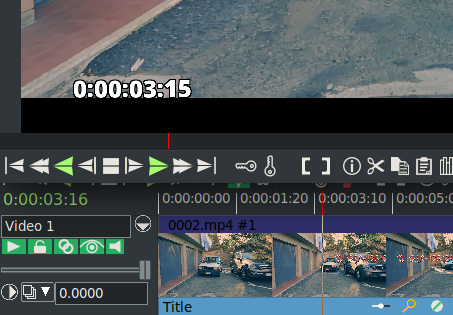
\includegraphics[width=0.6\linewidth]{cursor01.png}};    
	\node [yshift=-29mm, xshift=-1cm,anchor=east] at (img1.north west) (Compositor) {Red cursor in Compositor};
	\node [yshift=-40mm, xshift=-1cm,anchor=east] at (img1.north west) (Timeline) {red cursor in Timeline};
	\draw [->, line width=1mm] (Compositor) edge  ([yshift=-29mm] img1.north west);
	\draw [->, line width=1mm] (Timeline) edge  ([yshift=-40mm] img1.north west);   
	\end{tikzpicture}    
	\caption{"Default" mode with red cursors}
	\label{fig:cursor01}
\end{figure}

Figure~\ref{fig:cursor02} using the \textit{Always show next frame} method where the frame in the compositor is the same one that would have shown with a seek; in this case play was in the forward direction.  Note that the insertion pointer in the main track canvas shows 03:16 and the compositor shows 03:16.  Also, the cursor/cursor tops in both windows is white.

\begin{figure}[htpb]
	\centering
	%\includegraphics[width=0.8\linewidth]{name.ext}
	\begin{tikzpicture}[scale=1, transform shape]
	\node (img1) [yshift=0cm, xshift=0cm, rotate=0] {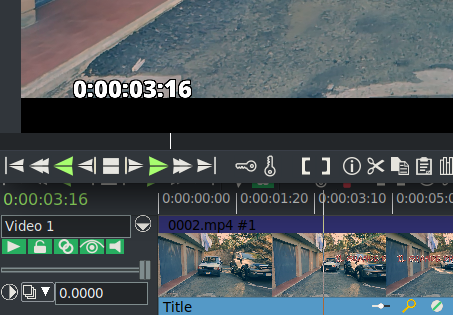
\includegraphics[width=0.6\linewidth]{cursor02.png}};    
	\node [yshift=-29mm, xshift=-1cm,anchor=east] at (img1.north west) (Compositor) {White cursor in Compositor};
	\node [yshift=-40mm, xshift=-1cm,anchor=east] at (img1.north west) (Timeline) {White cursor in Timeline};
	\draw [->, line width=1mm] (Compositor) edge  ([yshift=-29mm] img1.north west);
	\draw [->, line width=1mm] (Timeline) edge  ([yshift=-40mm] img1.north west);    
	\end{tikzpicture}    
	\caption{"Always show next frame" mode with white cursors}
	\label{fig:cursor02}
\end{figure}

\subsection{Seeking Issues}%
\label{sub:seeking_issue}

If you have an issue playing a video and not seeing it in the Compositor (just see a black screen), it is most likely due to the media not being designed to be \textit{editable}.  It is most likely not damaged.  Generally it just does not have keyframes which are needed for seeking which is what is done when you move around the media and start playing in the middle.  The media plays just fine in the compositor if you always play from the beginning because then you don’t need keyframes to seek.  You can get around this problem if you proxy the media.  A good choice to use for the proxy would be \textit{use scalar}, \textit{ffmpeg/mp4} and size of $\frac{1}{2}$.  The proxied media can then seek and you will see it play in the compositor because keyframes exist.

\section{Color Space and Color Range Affecting Playback}%
\label{sec:color_space_range_playback}

Playback \textit{single step} and \textit{plugins} cause the render to be in the session color model, while continuous playback with no plugins tries to use the file’s best color model for the display (for speed).
This can create a visible effect of a switch in color in the Compositor, usually shown as grayish versus over-bright.

The cause of the issue is that X11 is RGB only and it is used to draw the \textit{refresh frame}.  So single step is always drawn in RGB.  To make a YUV frame into RGB, a color model transfer function is used.  The math equations are based on color\_space and color\_range.  In this case, color\_range is the cause of the \textit{gray} offset.  The \textit{YUV mpeg} color range is $[16..235]$ for Y, $[16..240]$ for UV, and the color range used by \textit{YUV jpeg} is $[0..255]$ for YUV.

\begin{wrapfigure}[11]{O}{0.5\textwidth} 
    \vspace{-2ex}
    \centering
    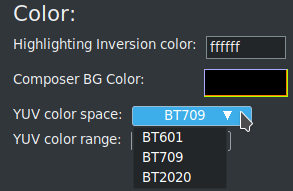
\includegraphics[width=0.5\textwidth,keepaspectratio]{color.png}
    \caption{Color space and Color range}
    \label{fig:color}
\end{wrapfigure} 

The mpeg YUV color range $[16..235]$ looks sort of like an old TV if it is viewed on a display with jpeg range $[0..255]$.  A common expression for the short \textit{mpeg} color range is \textit{compressed} color range.  If you are using color compressed data with no display decompression, or using uncompressed data and the display is configured to use compression, the color range will appear \textit{squished} or \textit{stretched}, as too gray or too much contrast.

The \textit{use X11 direct when possible} preference with X11 as your video driver, generally means that you value speed over color range.  When you use this feature and the color range preference is mismatched, the color switch offsets will still appear.  This is a personal choice solely for improved speed.

There is now program code to look for RGB versus YUV color model mismatches.  You can override the default setup, which mirrors the original code, via the following.

\texttt{Settings $\rightarrow$ Preferences $\rightarrow$ Appearance} tab in the lower left hand corner (Figure~\ref{fig:color}):

\begin{description}
    \item[YUV color space] default choice is BT601, alternate is BT709 (High Definition), BT2020 (UHD)
    \item[YUV color range] default choice is JPEG,   alternate is MPEG
\end{description}

\section{Automatic "Best Model" Media Load}%
\label{sec:conform_the_project}
When you load media with the insertion strategy of \textit{replace current project}, the program code will
automatically use the "best model" for the render based on the media's codec.  The best model is pretty
much going to be what works well for television.  This automation was added to facilitate easy use of
\CGG{}.  Which is to say that it is difficult for a new or occasional user to set all of the 
necessary parameters as best as possible so the program does it for you.  This means you do not have to 
\textit{conform your project} which ordinarily would have to have been done in the Resources window with RMB
click on the highlighted media and choosing \textit{Match project size}. 

However, this automatic method leads to the dilemma of where you have a 10-bit media file and it would
get loaded as RGBA-8 when you would prefer it to be RGBA-Float.  So instead of using \textit{replace current
project} when loading your media, you would have to make sure the project is first set to your desired
Format.  This could be done with the File$\rightarrow$New project and then setting your Color
Model to RGBA-Float and whatever other parameters you want.  Next when doing a File$\rightarrow$Load, use
\textit{Append in new tracks} or \textit{Create resources only}. This avoids using the "best model"
technique and uses instead what you have designated so that if you set the Color Model to RGBA-Float that
will be in effect.

It is important to note that even when using the "best model" no bits are lost if the input media is 10-bit
and the Color Model is RGBA-8. This is because the media will be loaded using the "case BC\_RGB16161616"
where 16 stands for 16 bits. It fills the other 6 bits not used for 10 bits with zeros.

\section{Simple Animation (Festival)}%
\label{sec:simple_animation_festival}

This functionality was added to \CGG{} by the original author to create simple animation.  The file type for this animation is \textit{Scene}.

To get started making a simple animated movie copy from the directory:\\
\texttt{<cin\_path>/cinelerra/tests} the \texttt{text2movie} and \texttt{text2movie.xml}. \\
You can see what this does via \texttt{File $\rightarrow$ Load\dots $\rightarrow$ text2movie.xml}.  The file text2movie acts like a normal asset, except changes to it are immediately reflected on the timeline without reloading and the length is infinite.  You can just edit the text2movie file to change the script.  If the length of the movie increases, drag the right edit handle to extend the edit or use the pulldown \texttt{Edit $\rightarrow$ edit length}. There is one audio channel created for every character.  The frame rate, sample rate, frame size, and camera angles are fixed.  To see these values, right click on the asset and look at the \textit{Asset info}.

Currently the functionality that is implemented focuses on dialog between two people.  The models are defined in model files saved in \CGG{}'s executable directory (for example, \texttt{/opt/cinelerra/models}).  The character model and voice is selected separately in the script.  The model files have the same name that appears in the script and are usually saved in the directory the script is in, but there is a defined search path, if not.  You can create new models for the script without affecting the entire system.  These models define the total size of the model along with the images used -- the model images are 2D png images because all the animations are baked.  Since there is no 3D renderer, no custom movement is supported.

There are currently 2 actions implemented:

\begin{enumerate}
    \item Character2 can cut off character1 if character1's dialog ends in “\dots”
    \item Inserting “[pause]” anywhere causes the character to pause.  This is useful for adjusting the timing of dialog.
\end{enumerate}

This is \textit{simple} animation so you can expect speech synthesis not to be that good.  And you will have to adjust punctuation and spelling based on the sound.  Since the dialog is rendered on-demand, there is a delay when each character starts to speak but you can split dialog into shorter blocks to reduce the delay.

\section{Textbox Non-std Character / Unicode Insertion}%
\label{sec:textbox_non_std_character_unicode}

If you want to enter a special character -- like a bullet, an accent grave character, or a mathematical summation symbol -- you can use the unicode equivalent in a textbox to do so.  In the textbox, keyin Ctrl-Shift-U which puts you into single character unicode mode, then keyin the numerical value for the intended single character followed by the carriage return.  For a voluminous list of possible special characters, you can go to {\small \url{https://unicode-table.com/en/}} on the internet to choose by highlighting a character to get its numerical equivalence.  For example, $U+2022$ is a bullet.  If you make a mistake, you can use the \textit{backspace} key or if you want to exit unicode-insert-mode, use the \textit{ESC} key.  This feature is especially useful with the \textit{Title} plugin and for naming Tracks in the main window.

However, it is worth mentioning that some special characters are available via the \textit{compose} key in the current distribution. {\small \url{https://en.wikipedia.org/wiki/Compose_key}}

